\documentclass[11pt]{article}

\usepackage[utf8]{inputenc}
\usepackage[T1]{fontenc}
\usepackage{lmodern}
\usepackage[margin=1in]{geometry}
\usepackage{amsmath,amssymb}
\usepackage{graphicx}
\usepackage{booktabs}
\usepackage{siunitx}
\usepackage{caption}
\usepackage{subcaption}
\usepackage{xcolor}
\usepackage[colorlinks=true,linkcolor=blue,citecolor=blue,urlcolor=blue]{hyperref}

% Figures live in ../results/figures relative to this file.
\graphicspath{{../results/figures/}{results/figures/}}

\title{\textbf{Detecting Sub-threshold Eavesdropping in BB84 Quantum Key
Distribution with Machine Learning}}
\author{Yash Yadav \\ \small Indian Institute of Technology Kanpur}
\date{\today}

\begin{document}
\maketitle

\begin{abstract}
The security of the BB84 quantum key distribution (QKD) protocol is conventionally
certified by a single statistic: if the quantum bit error rate (QBER) exceeds the
$\sim$11\% threshold, the key is discarded. We show that this operational test is
blind to a class of \emph{sub-threshold} eavesdropping attacks that hold the QBER
below the alarm level while leaving distinct statistical fingerprints elsewhere in
the channel. Using a photon-number/decoy-state BB84 simulator --- validated against
closed-form QKD theory --- we model two such attacks: a basis-biased
intercept--resend attack (per-basis QBER asymmetry) and a \emph{gain-matched}
photon-number-splitting (PNS) attack (decoy-gain collapse at normal QBER and normal
signal gain). The operational QBER test detects \SI{0.8}{\percent} of these attacks;
a random forest on a richer feature set detects \SI{87}{\percent} (AUC $0.96$). The
gain-matched PNS attack is \emph{invisible} to QBER (AUC $0.51$, i.e.\ random) yet
detected perfectly (AUC $1.00$) through the decoy/signal gain ratio alone, exactly as
decoy-state theory predicts. Finally, a quantum-kernel SVM with a naive encoding
fails (AUC $0.58$) due to exponential kernel concentration, but becomes competitive
with classical baselines once the encoding is tuned (AUC $0.95$) --- competitive, but
with no quantum advantage on this low-dimensional task.
\end{abstract}

\section{Introduction}
Quantum key distribution lets two parties, Alice and Bob, share a secret key whose
security rests on physics rather than computational hardness. In BB84~\cite{bb84},
Alice sends qubits in one of two conjugate bases and Bob measures in a randomly
chosen basis; after public basis reconciliation (\emph{sifting}), the residual
disagreement rate --- the QBER --- bounds an eavesdropper's information. The textbook
security check is a threshold: if QBER $>\sim$11\%, eavesdropping is assumed and the
key is aborted~\cite{shorpreskill}.

This single-number test only sees the \emph{average} error rate. A sophisticated
eavesdropper can deliberately keep the QBER below the threshold while still disturbing
the channel in ways that are statistically detectable in other observables. We ask:
\textbf{can machine learning detect eavesdropping that the QBER threshold misses?}
We answer affirmatively, identify which physical observables carry the signal, and
report an honest assessment of whether a quantum kernel helps.

\section{Background}
\paragraph{The QBER threshold.} For symmetric intercept--resend each intercepted
qubit incurs a 25\% error, so a full attack drives QBER to $\sim$25\%, far above the
bound. The threshold test is effective against such overt attacks but assumes the
eavesdropper operates near full strength.

\paragraph{Basis-biased intercept--resend.} If Eve intercepts only a fraction of
pulses and always measures in a fixed basis ($Z$), her errors concentrate in the
conjugate ($X$) basis. The \emph{total} QBER stays below 11\%, but the per-basis rates
become asymmetric, $\mathrm{QBER}_X \gg \mathrm{QBER}_Z$ --- a signature the averaged
test discards.

\paragraph{PNS and decoy states.} Real sources emit weak coherent pulses with a
Poissonian photon number; some pulses contain $\ge 2$ photons. In a PNS attack Eve
blocks single-photon pulses and splits one photon from each multi-photon pulse,
forwarding the rest. Crucially, a competent Eve forwards through a \emph{lossless}
line and throttles her forwarding so that Bob's \emph{signal gain matches} the
expected lossy value --- masking her interference. She adds no error (she does not
measure--resend), so QBER is unchanged too. Because she cannot distinguish signal
from decoy pulses, the same throttling is applied to low-intensity \emph{decoy}
pulses, whose multi-photon fraction is far smaller; their gain therefore
collapses~\cite{decoy}. The decoy/signal gain ratio is the \emph{only} remaining
signature --- which is precisely why decoy-state QKD was invented.

\section{Methods}
\subsection{Simulator}
We extend a Qiskit-Aer BB84 simulator with a photon-number/decoy-state channel.
Each pulse is randomly signal ($\mu_s=0.5$) or decoy ($\mu_d=0.1$), each with
probability tuned by \texttt{decoy\_prob}$=0.5$; its photon number is
$k\sim\mathrm{Poisson}(\mu)$ and it is detected with probability $1-(1-\eta)^k$ at
transmittance $\eta=0.15$ (a high-loss channel, the regime where PNS is a genuine
threat). Detected qubits are prepared, sent through a depolarizing channel (3\% gate
error), and measured on a real single-qubit circuit. The simulator returns total and
per-basis QBER, the sift ratio, and the signal/decoy gains. Bob's measurement sampler
is seeded, so all results are reproducible.

For the gain-matched PNS attack, Eve forwards multi-photon pulses with probability
$q = (1-e^{-\mu_s\eta}) / P(k\ge 2\mid\mu_s)$, which makes the observed signal gain
equal the legitimate value $1-e^{-\mu_s\eta}$.

\subsection{Theory validation}
Before any learning, we checked the simulator against closed-form QKD expressions
(Table~\ref{tab:theory}); all observables agree to within sampling error.

\begin{table}[h]
  \centering
  \caption{Simulator vs.\ theory ($\mu_s{=}0.5,\ \mu_d{=}0.1,\ \eta{=}0.15$).}
  \label{tab:theory}
  \begin{tabular}{lcc}
    \toprule
    Observable & Simulated & Theory \\
    \midrule
    Secure signal gain $1-e^{-\mu_s\eta}$        & 0.223 & 0.221 \\
    Secure decoy/signal ratio                    & 0.215 & 0.221 \\
    PNS signal gain $P(k\ge2\mid\mu_s)$          & 0.089 & 0.090 \\
    PNS decoy/signal ratio                       & 0.055 & 0.052 \\
    Secure QBER (3\% depolarizing)               & 0.020 & 0.02--0.03 \\
    Biased-IR asymmetry ($\approx$ strength/2)   & 0.115 & 0.100 \\
    \bottomrule
  \end{tabular}
\end{table}

\subsection{Attacks, features, models}
The basis-biased attack intercepts a fraction $p\in[0.08,0.22]$ of pulses (chosen to
keep total QBER below 11\%); PNS is gain-matched as above. Each session yields five
features: total QBER, per-basis QBER asymmetry $|\mathrm{QBER}_Z-\mathrm{QBER}_X|$,
signal gain, decoy/signal gain ratio, and sift ratio. We train logistic regression, a
random forest, and an SVM (classical), and a quantum-kernel SVM using a
\texttt{ZZFeatureMap} fidelity kernel $K(x_i,x_j)=|\langle\phi(x_i)|\phi(x_j)\rangle|^2$
computed exactly from statevectors. The dataset has 800 sessions of 6000 pulses each
(attack ratio $0.47$); results use 5-fold stratified cross-validation.

\section{Results}
\paragraph{All attacks are sub-threshold.} Figure~\ref{fig:subthreshold} shows the
secure and attacked QBER distributions overlapping below the 11\% line: only
\SI{0.8}{\percent} of attack sessions exceed the threshold, so the operational test
flags essentially none.

\begin{figure}[t]
  \centering
  \begin{subfigure}{0.48\textwidth}
    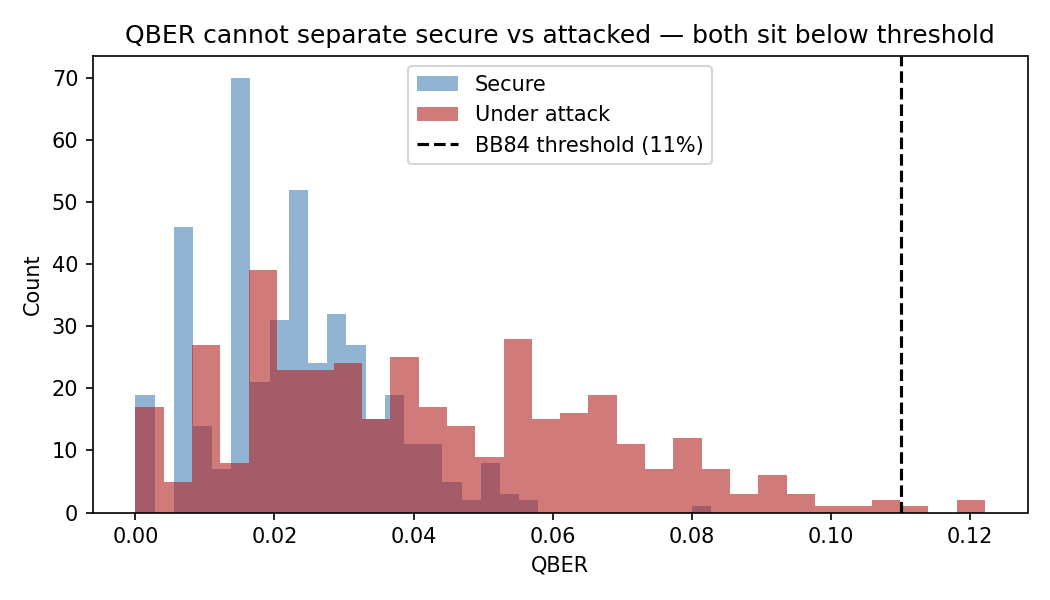
\includegraphics[width=\linewidth]{subthreshold_qber.png}
    \caption{QBER cannot separate the classes.}
    \label{fig:subthreshold}
  \end{subfigure}\hfill
  \begin{subfigure}{0.48\textwidth}
    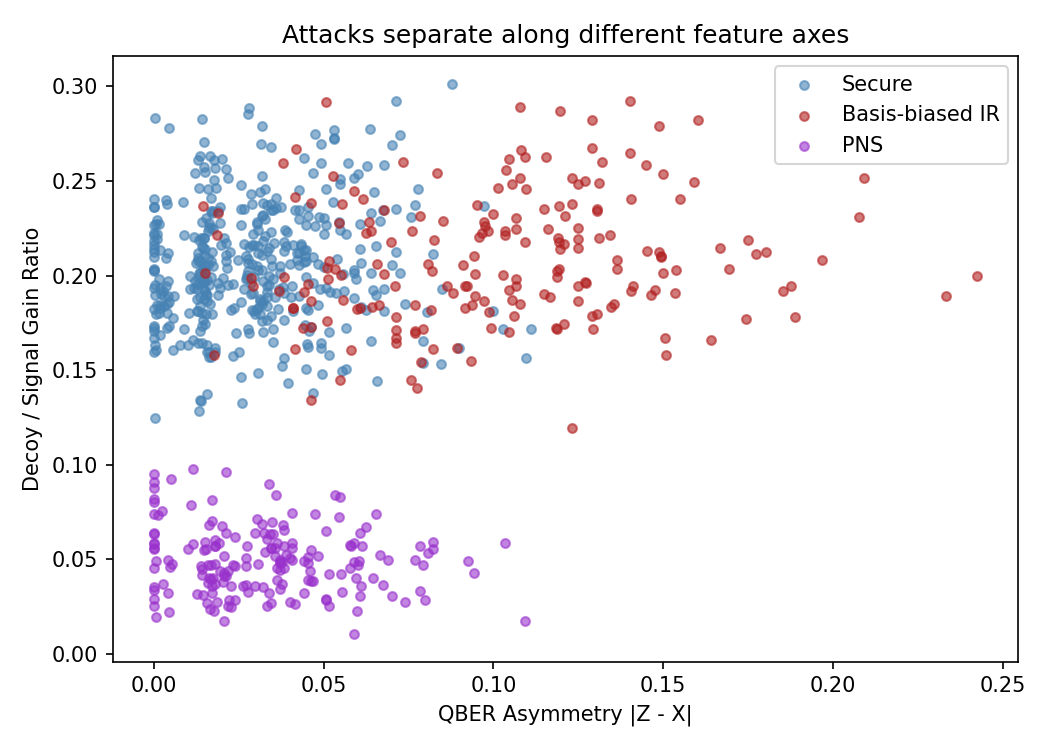
\includegraphics[width=\linewidth]{feature_separation.png}
    \caption{The attacks separate along other axes.}
    \label{fig:separation}
  \end{subfigure}
  \caption{Left: secure (blue) and attacked (red) sessions have overlapping,
  sub-threshold QBER. Right: basis-biased and PNS attacks are cleanly separable in the
  (asymmetry, decoy-ratio) plane.}
\end{figure}

\paragraph{Headline: threshold vs.\ ML.} Table~\ref{tab:headline} and
Figure~\ref{fig:headline} contrast the operational QBER test with the random forest:
\SI{0.8}{\percent} detection (AUC $0.726$) versus \SI{87.4}{\percent} (AUC $0.963$).

\begin{table}[h]
  \centering
  \caption{Detection performance (5-fold cross-validated).}
  \label{tab:headline}
  \begin{tabular}{lcc}
    \toprule
    Detector & Detection rate @ 11\% & ROC AUC \\
    \midrule
    QBER threshold test    & \SI{0.8}{\percent}  & 0.726 \\
    ML (rich features)     & \SI{87.4}{\percent} & 0.963 \\
    \bottomrule
  \end{tabular}
\end{table}

\begin{figure}[t]
  \centering
  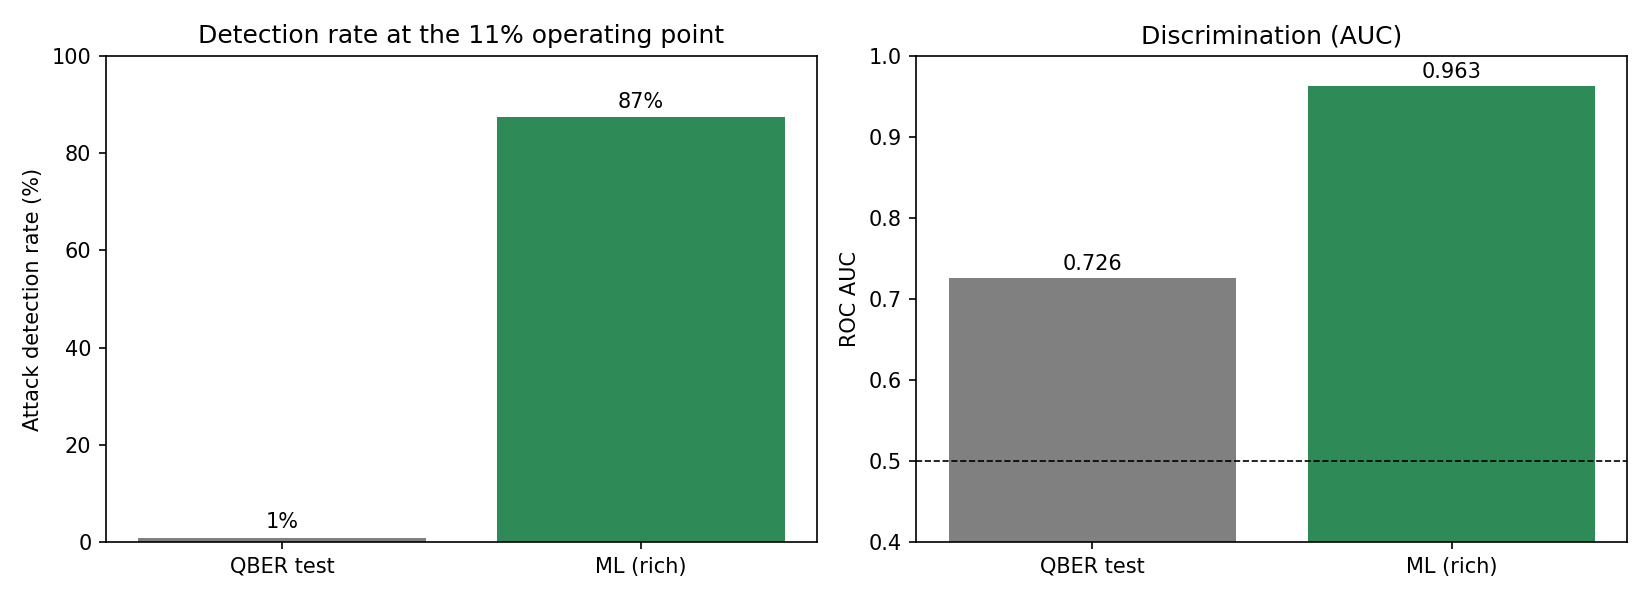
\includegraphics[width=0.8\textwidth]{threshold_vs_ml.png}
  \caption{QBER threshold test (gray) versus ML on the full feature set (green):
  detection rate at the 11\% operating point (left) and overall AUC (right).}
  \label{fig:headline}
\end{figure}

\paragraph{Per-attack analysis.} Table~\ref{tab:perattack} decomposes the result. The
basis-biased attack raises QBER as a continuous score (AUC $0.931$) but stays below
the alarm level, so the operational threshold still misses it. The gain-matched PNS
attack is the decisive case: QBER carries \emph{no} signal (AUC $0.508$, random) and
neither does the signal gain (AUC $0.57$), yet ML detects it perfectly (AUC $1.000$)
through the decoy ratio alone.

\begin{table}[h]
  \centering
  \caption{Secure-vs-attack discrimination, by attack family.}
  \label{tab:perattack}
  \begin{tabular}{lcc}
    \toprule
    Attack & QBER-only AUC & ML AUC \\
    \midrule
    Basis-biased intercept--resend & 0.931 & 0.930 \\
    Gain-matched PNS               & 0.508 & 1.000 \\
    \bottomrule
  \end{tabular}
\end{table}

\paragraph{Feature importance and classical baselines.} The random forest concentrates
its importance on the QBER asymmetry and the decoy ratio, not QBER itself
(Fig.~\ref{fig:importance}). The classical models are comparable (LogReg AUC
$0.954\pm0.012$, RF $0.963\pm0.008$, SVM $0.956\pm0.013$); ROC curves in
Figure~\ref{fig:roc}.

\begin{figure}[t]
  \centering
  \begin{subfigure}{0.48\textwidth}
    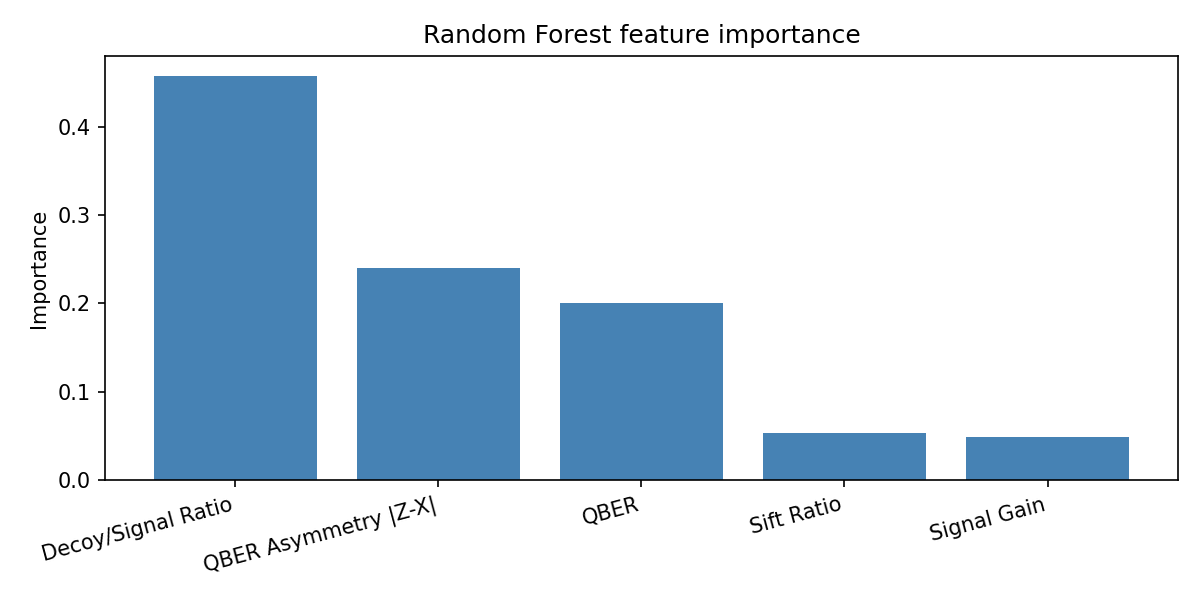
\includegraphics[width=\linewidth]{feature_importance.png}
    \caption{Feature importance.}
    \label{fig:importance}
  \end{subfigure}\hfill
  \begin{subfigure}{0.48\textwidth}
    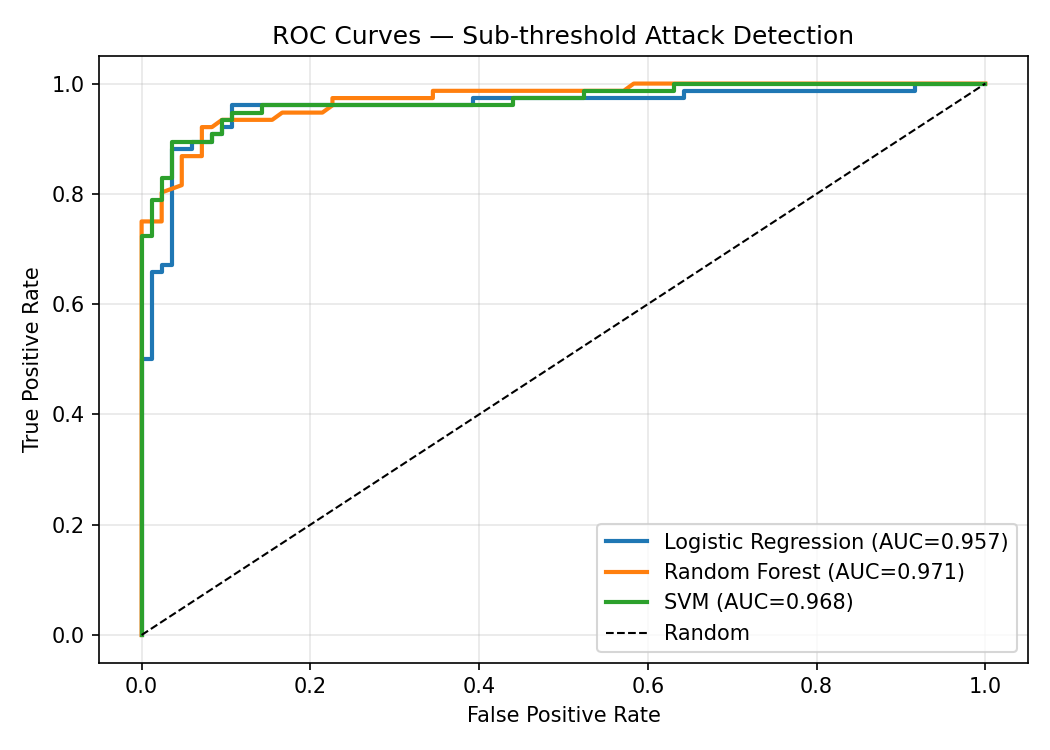
\includegraphics[width=\linewidth]{roc_curves.png}
    \caption{Classical ROC curves.}
    \label{fig:roc}
  \end{subfigure}
  \caption{QBER is weak; the asymmetry and decoy ratio carry the signal.}
\end{figure}

\paragraph{Classical vs.\ quantum, and kernel concentration.} On an identical $n=150$
training set the classical models reach AUC $0.94$--$0.965$
(Fig.~\ref{fig:fair}). A naively-encoded quantum kernel ($[0,\pi]$ angles, two
repetitions) collapses to AUC $0.577$: its kernel matrix is nearly the identity
(off-diagonal mean $0.04$) because the data states become near-orthogonal ---
\emph{exponential kernel concentration}. Shrinking the encoding angles to $[0,\pi/8]$
with a single repetition restores AUC $0.950$ (Fig.~\ref{fig:tuning}), competitive
with classical but offering no advantage.

\begin{figure}[t]
  \centering
  \begin{subfigure}{0.48\textwidth}
    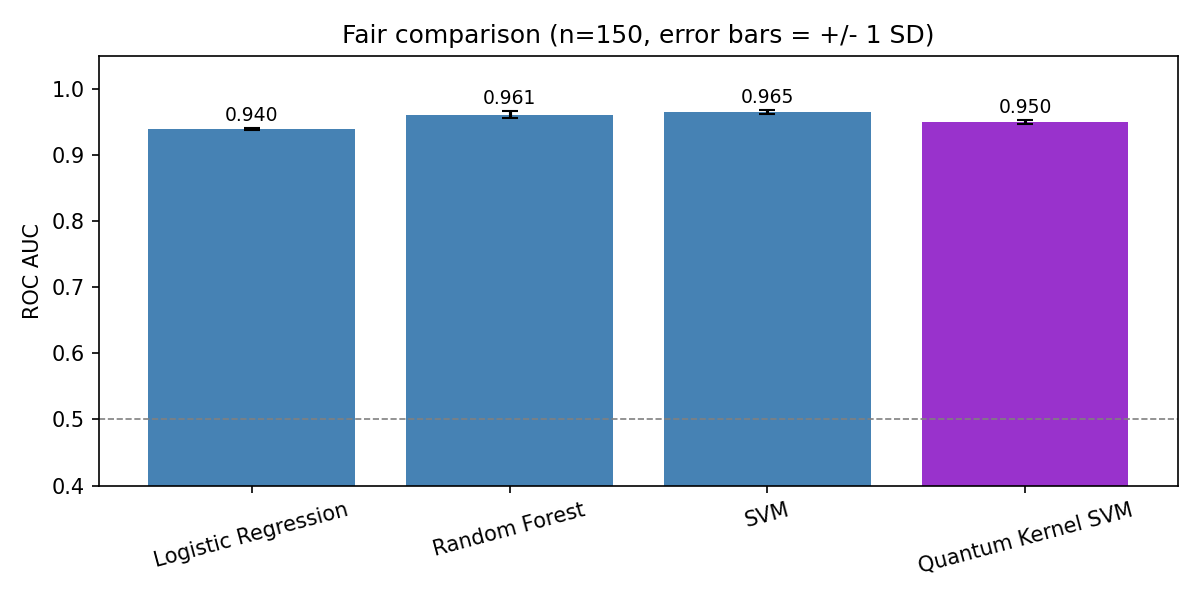
\includegraphics[width=\linewidth]{fair_comparison.png}
    \caption{Fair comparison ($n=150$).}
    \label{fig:fair}
  \end{subfigure}\hfill
  \begin{subfigure}{0.48\textwidth}
    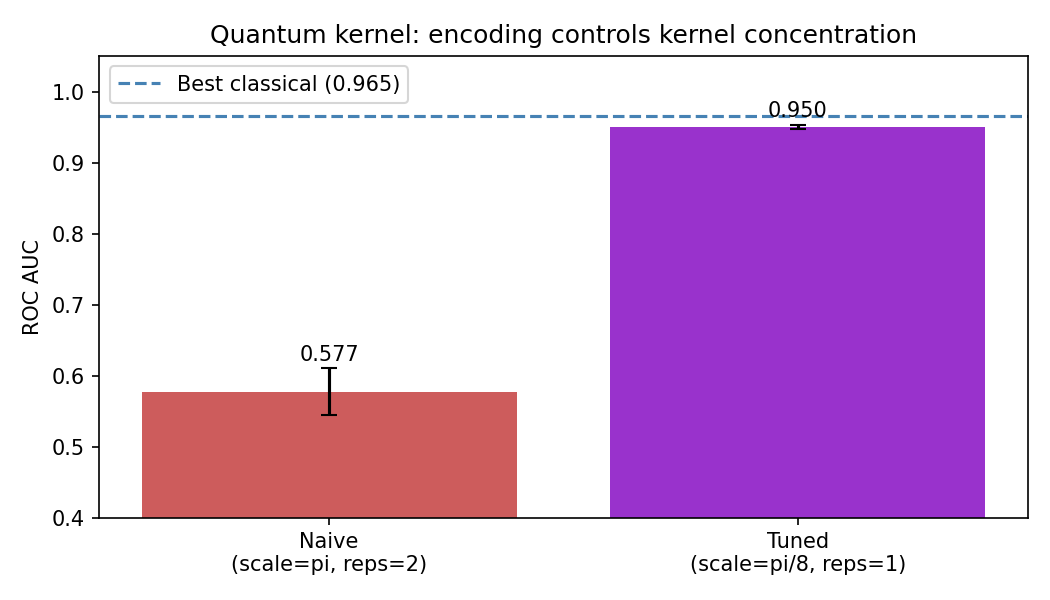
\includegraphics[width=\linewidth]{quantum_tuning.png}
    \caption{Encoding controls concentration.}
    \label{fig:tuning}
  \end{subfigure}
  \caption{The quantum-kernel SVM matches classical only after the encoding is tuned
  to avoid exponential concentration ($0.58 \rightarrow 0.95$).}
\end{figure}

\section{Discussion}
The central finding is operationally meaningful: the BB84 QBER threshold, used in
practice as a go/no-go check, fails against attacks engineered to sit below it,
whereas a lightweight classifier on already-available channel statistics recovers
them. The attack mechanisms (basis bias, PNS) are known; the contribution is the
demonstration that \emph{cheap multivariate monitoring closes a detection gap the
threshold leaves open}, with the per-basis asymmetry and decoy ratio identified as the
informative observables. The gain-matched PNS result reproduces, through a data-driven
lens, the exact reason decoy-state QKD exists.

We also report two honest negatives. A naive quantum kernel \emph{fails} on this task
due to exponential concentration; only after tuning does it match (never beat)
classical methods --- consistent with the literature on quantum kernels for
low-dimensional classical data. We present this plainly rather than selecting a
favourable configuration.

\paragraph{Limitations.} The photon model is a simplified Monte-Carlo abstraction (no
dark counts, after-pulsing, or finite-key corrections), the noise is idealised
depolarizing, and only two attack families are studied. Extending to finite-key
statistics, additional attacks (Trojan-horse, time-shift), and raw time-series
features are natural next steps.

\section{Conclusion}
Sub-threshold eavesdropping defeats the standard BB84 QBER test but not machine
learning on richer channel statistics: a random forest detects \SI{87}{\percent} of
attacks that the threshold catches at \SI{0.8}{\percent}, and detects gain-matched PNS
--- invisible to both QBER and signal gain --- perfectly via the decoy ratio. A
quantum kernel offers no advantage and fails outright if naively configured. The work
argues for treating QKD eavesdropping detection as a multivariate statistical problem
rather than a single-threshold check.

\begin{thebibliography}{9}
\bibitem{bb84} C.\ H.\ Bennett and G.\ Brassard, ``Quantum cryptography: Public key
distribution and coin tossing,'' \emph{Proc.\ IEEE Int.\ Conf.\ Computers, Systems and
Signal Processing}, 1984.
\bibitem{shorpreskill} P.\ W.\ Shor and J.\ Preskill, ``Simple proof of security of the
BB84 quantum key distribution protocol,'' \emph{Phys.\ Rev.\ Lett.} \textbf{85}, 441
(2000).
\bibitem{decoy} H.-K.\ Lo, X.\ Ma, and K.\ Chen, ``Decoy state quantum key
distribution,'' \emph{Phys.\ Rev.\ Lett.} \textbf{94}, 230504 (2005).
\end{thebibliography}

\end{document}
